\RequirePackage{luatex85}
\documentclass{standalone}
\usepackage{amssymb,amsmath}
\usepackage{tikz}
\usetikzlibrary{automata,positioning}
\begin{document}
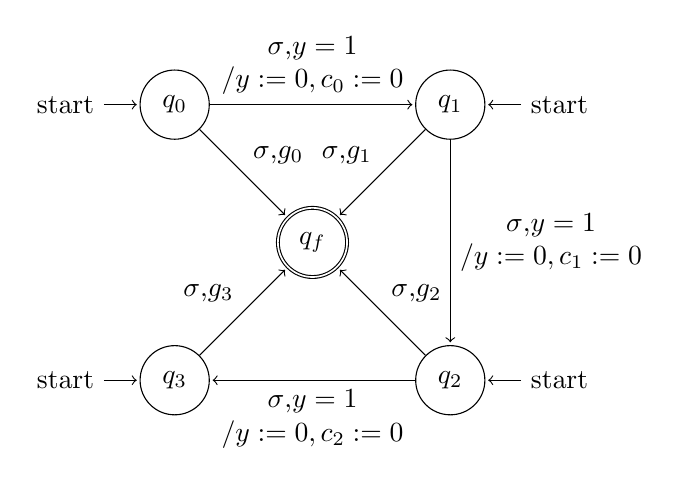
\begin{tikzpicture}[shorten >=1pt,node distance=3.5cm,on grid,auto] 
 \node[state,initial] (q_0) {$q_0$};
 \node[state,initial right] (q_1)[right=of q_0] {$q_1$};
 \node[state,initial right] (q_2)[below=of q_1] {$q_2$};
 \node[state,initial] (q_3)[below=of q_0] {$q_3$};
 \node[state,accepting] (q_f) at (1.75,-1.75) {$q_f$};
 \path[->]
 (q_0) edge node[align=center] {$\sigma$,$y=1$\\ $/y:=0,c_0:=0$} (q_1)
 (q_1) edge node[align=center] {$\sigma$,$y=1$\\ $/y:=0,c_1:=0$} (q_2)
 (q_2) edge node[align=center] {$\sigma$,$y=1$\\ $/y:=0,c_2:=0$} (q_3)

 (q_0) edge node[align=center] {$\sigma$,$g_0$} (q_f)
 (q_1) edge[above left] node[align=center] {$\sigma$,$g_1$} (q_f)
 (q_2) edge[above right] node[align=center] {$\sigma$,$g_2$} (q_f)
 (q_3) edge node[align=center] {$\sigma$,$g_3$} (q_f);
\end{tikzpicture}
 \end{document}